% vim: set spell spelllang=es syntax=tex :

\documentclass[11pt,a4paper,spanish]{beamer}

\usepackage[spanish]{babel}

\usepackage[utf8]{inputenc}

\usepackage{graphicx}

\usepackage{subcaption} %Para Subfigure

\usepackage{caption} %Para captions en las figuras sin prefijo

\usepackage{ccicons}

\usepackage{url}

\usepackage{babelbib}

\usefonttheme{serif}

\setlength{\parskip}{1.5mm}

\newcommand{\codeword}[1]{\mbox{\texttt{\textcolor{blue}{#1}}}}

\usetheme{Rochester}
\usecolortheme{whale}

%\usetheme{Warsaw}

\beamertemplatenavigationsymbolsempty

\setbeamertemplate{background canvas}{
    \raisebox{-0.99\paperheight}[0pt][0pt]{
        \makebox[\paperwidth]{
            \null
            \hspace{-1em}
            
\includegraphics[width=0.09\paperwidth]{logos/fai.pdf}
            \hspace{0.8\paperwidth}
            %\hfill
            \hspace{-1em}
            \includegraphics[width=0.09\paperwidth]{logos/uncoma.pdf}
            }
    }
}

\title{Introducción a\\
\textbf{Introducción a la\\
Administración de sistemas}}

\author{}

\date{}

\defbeamertemplate{footline}{centered page number}
{
    \hspace*{\fill}
    \usebeamercolor[fg]{blue}
    \usebeamerfont{page number in head/foot}
    \insertpagenumber\,/\,\insertpresentationendpage
    \hspace*{\fill}\vskip2pt
}
\setbeamertemplate{footline}[centered page number]

\begin{document}

\begin{frame}[noframenumbering]

    \maketitle
    \centering
    \vspace{-8em}~
    \begin{figure}
    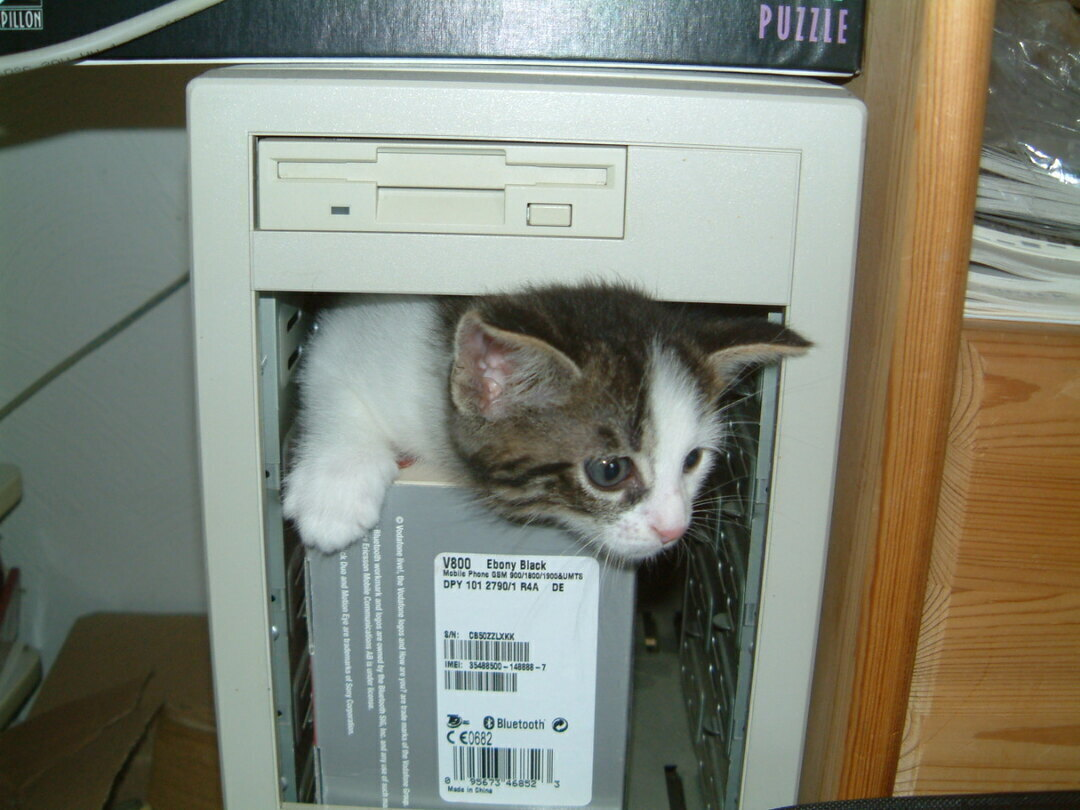
\includegraphics[height=0.55\textheight]{img/ckitten.jpg}
        \captionsetup{textfont=tiny,labelformat=empty}
        \caption{\ccbysa\cite{ckitten}}
    \end{figure}

\end{frame}

\begin{frame}

    \frametitle{Temario}

\begin{itemize}

\item ¿Quiénes?

\item ¿Qué?

\item ¿Cuándo y dónde?

\item ¿Cómo?

\end{itemize}

\end{frame}

\begin{frame}

    \frametitle{Equipo de cátedra}

\begin{itemize}

\item Docentes a cargo:
    \begin{itemize}
        \item Rodrigo S. Cañibano
        \item Javier Forquera
    \end{itemize}
\end{itemize}

\end{frame}

\begin{frame}

    \frametitle{Programa de la materia}

\begin{enumerate}
    \item \textbf{Introducción al intérprete de línea de comandos.}
    \item \textbf{Sistemas de archivos.}
    \item \textbf{Administración de Usuarios.}
    \item \textbf{Proceso de encendido y apagado.}
\end{enumerate}

\end{frame}

\begin{frame}

    \frametitle{Programa de la materia}

\begin{enumerate}
    \item \textbf{Introducción al intérprete de línea de comandos:}
        \begin{itemize}
            \item Definición.
            \item Ordenes básicas.
            \item Variables de entorno.
            \item Uso de los manuales en línea.
            \item Comodines y redirección.
            \item Editor de texto Vim.
        \end{itemize}
\end{enumerate}

\end{frame}

\begin{frame}

    \frametitle{Programa de la materia}

\begin{enumerate}
    \setcounter{enumi}{1}
    \item \textbf{Sistemas de archivos:}
        \begin{itemize}
            \item Estándar de Jerarquía de Sistemas de Archivos en sistemas
                GNU/Linux.
            \item Órdenes del intérprete de líneas de comandos, relativas a
                sistemas de archivos.
            \item Introducción a los permisos de archivos.
            \item Tipos de archivos en GNU/Linux.
            \item Formato interno de archivos regulares.
        \end{itemize}
\end{enumerate}

\end{frame}

\begin{frame}

    \frametitle{Programa de la materia}

\begin{enumerate}
    \setcounter{enumi}{2}
    \item \textbf{Administración de Usuarios:}
        \begin{itemize}
            \item Concepto de usuario.
            \item Concepto de sistema multiusuario.
            \item Administración de usuarios mediante herramientas
                específicas.
        \end{itemize}
\end{enumerate}

\end{frame}

\begin{frame}

    \frametitle{Programa de la materia}

\begin{enumerate}
    \setcounter{enumi}{3}
    \item \textbf{Proceso de encendido y apagado:}
        \begin{itemize}
            \item Elementos de software involucrados en el encendido y apagado
                de una máquina.
            \item Concepto de nivel de ejecución.
            \item Herramientas para la administración de niveles de ejecución.
        \end{itemize}
\end{enumerate}

\end{frame}

\begin{frame}

    \frametitle{Página del curso de la materia en \emph{PEDCO}}
    \framesubtitle{\url{https://pedco.uncoma.edu.ar/course/view.php?id=1556}}

\begin{itemize}
    \item Últimas novedades.
    \item Información de contacto de los docentes.
    \item Horarios.
    \item Programa de la materia.
    \item Trabajos prácticos.
    \item Foros:
        \begin{itemize}
            \item Novedades.
            \item Consultas.
        \end{itemize}
\end{itemize}

\end{frame}

\begin{frame}

    \frametitle{Página del curso de la materia en \emph{PEDCO}}
    \framesubtitle{\url{https://pedco.uncoma.edu.ar/course/view.php?id=1556}}

\begin{itemize}
    \item Deben configurar para que les lleguen los mensajes a su correo:
    \begin{figure}
        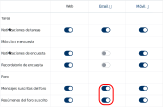
\includegraphics[height=0.65\textheight]{img/conf_pedco.pdf}
        \captionsetup{textfont=tiny,labelformat=empty}
        \caption{\url{}https://pedco.uncoma.edu.ar/message/notificationpreferences.php?userid=3052}
    \end{figure}
\end{itemize}

\end{frame}

\begin{frame}

    \frametitle{SIU Guaraní}
    \framesubtitle{\url{https://siufai.uncoma.edu.ar/}}

\begin{itemize}
    \item Sistema de Gestión Académica Guaraní.
    \item Inscribirse a materias y exámenes finales.
    \item Consultar el plan de la carrera.
    \item Consultar la historia académica.
    \item Actualizar datos personales.
\end{itemize}

\textbf{¡Si no están anotados en el \emph{SIU Guaraní} no están anotados a la
    materia!}

\end{frame}

\begin{frame}

    \frametitle{Metodología}
    \framesubtitle{Clases}

\begin{itemize}
    \item Clases teóricas:
    \begin{itemize}
        \item Jueves \textbf{18:00hs} a \textbf{20:00hs} (\textbf{Laboratorio
            biblioteca}).
    \end{itemize}
    \item Clases prácticas:
    \begin{itemize}
        \item Viernes \textbf{19:00hs} a \textbf{21:00hs} (\textbf{Laboratorio
            3}).
    \end{itemize}

\end{itemize}

\end{frame}

\begin{frame}

    \frametitle{Metodología}
    \framesubtitle{Trabajos prácticos y exámenes}

\begin{itemize}

    \item Ejercitación en computadora.
    \item Pueden conectarse a las máquinas de los laboratorios por
        \emph{ssh}:\\
        \codeword{ssh \$USER@aula-ssh.fi.uncoma.edu.ar -p 60173}
        \begin{itemize}
            \item[] \tiny{\emph{(Remplazar \codeword{\$USER} por su usuario de
                laboratorio)}}
        \end{itemize}
    \item Los trabajos prácticos no se entregan, ni son corregidos por la
        cátedra.
        \begin{itemize}
            \item Se recomienda igualmente hacerlos de la forma más prolija
                posible ya que serán el documento principal para estudiar para
                los exámenes.
        \end{itemize}

\end{itemize}

\end{frame}

\begin{frame}

    \frametitle{Metodología}
    \framesubtitle{Cursar la materia}

\begin{itemize}

    \item Aprobar los dos exámenes parciales (o sus respectivos
        recuperatorios).
    \item Cada parcial se aprueba teniendo un $60\%$ de las respuestas
        correctas.
    \item Se evalúan los contenidos prácticos y teóricos vistos en los
        trabajos prácticos.
        %Se pueden consultar los trabajos prácticos resueltos.
    \item Los exámenes recuperatorios se llevaran a cabo al final del
        cuatrimestre.

\end{itemize}

\end{frame}

\begin{frame}

    \frametitle{Metodología}
    \framesubtitle{Promocionar la materia}

\begin{itemize}

    \item Si se aprueban ambos exámenes con una nota superior a $80\%$, se
        promociona la materia.
        \begin{itemize}
            \item \emph{¡Los recuperatorios cuentan! Y se puede rendir
                el recuperatorio para subir la nota.}
        \end{itemize}

\end{itemize}

\end{frame}

\begin{frame}

    \frametitle{Metodología}
    \framesubtitle{Fechas TENTATIVAS}

\begin{itemize}

    \item Primer examen parcial: \textbf{Jueves 08} de Mayo.
    \item Segundo examen parcial: \textbf{Viernes 06} de Junio.
    \item Recuperatorio del primer examen parcial: \textbf{Viernes 13} de
        Junio.
    \item Recuperatorio del segundo examen parcial: \textbf{Viernes 26} de
        Junio.

\end{itemize}

\end{frame}

\begin{frame}

    \frametitle{Finalizando}

\begin{itemize}

\item ¿Quiénes?

\item ¿Qué?

\item ¿Cuándo y dónde?

\item ¿Cómo?

\end{itemize}

\end{frame}

\begin{frame}

\title{¿Consultas?}
\maketitle

\end{frame}

\newcounter{lastPage}
\setcounter{lastPage}{\number\value{page}}

\begin{frame}%[allowframebreaks]

\frametitle{Atribuciones}

\bibliographystyle{abbrv}
\setbeamertemplate{bibliography item}{\insertbiblabel}
\tiny
\bibliography{refimg}
\end{frame}

\setcounter{page}{\number\value{lastPage}}

\end{document}
